% Options for packages loaded elsewhere
\PassOptionsToPackage{unicode}{hyperref}
\PassOptionsToPackage{hyphens}{url}
\PassOptionsToPackage{dvipsnames,svgnames,x11names}{xcolor}
%
\documentclass[
  letterpaper,
  DIV=11,
  numbers=noendperiod]{scrartcl}

\usepackage{amsmath,amssymb}
\usepackage{iftex}
\ifPDFTeX
  \usepackage[T1]{fontenc}
  \usepackage[utf8]{inputenc}
  \usepackage{textcomp} % provide euro and other symbols
\else % if luatex or xetex
  \usepackage{unicode-math}
  \defaultfontfeatures{Scale=MatchLowercase}
  \defaultfontfeatures[\rmfamily]{Ligatures=TeX,Scale=1}
\fi
\usepackage{lmodern}
\ifPDFTeX\else  
    % xetex/luatex font selection
\fi
% Use upquote if available, for straight quotes in verbatim environments
\IfFileExists{upquote.sty}{\usepackage{upquote}}{}
\IfFileExists{microtype.sty}{% use microtype if available
  \usepackage[]{microtype}
  \UseMicrotypeSet[protrusion]{basicmath} % disable protrusion for tt fonts
}{}
\makeatletter
\@ifundefined{KOMAClassName}{% if non-KOMA class
  \IfFileExists{parskip.sty}{%
    \usepackage{parskip}
  }{% else
    \setlength{\parindent}{0pt}
    \setlength{\parskip}{6pt plus 2pt minus 1pt}}
}{% if KOMA class
  \KOMAoptions{parskip=half}}
\makeatother
\usepackage{xcolor}
\setlength{\emergencystretch}{3em} % prevent overfull lines
\setcounter{secnumdepth}{-\maxdimen} % remove section numbering
% Make \paragraph and \subparagraph free-standing
\makeatletter
\ifx\paragraph\undefined\else
  \let\oldparagraph\paragraph
  \renewcommand{\paragraph}{
    \@ifstar
      \xxxParagraphStar
      \xxxParagraphNoStar
  }
  \newcommand{\xxxParagraphStar}[1]{\oldparagraph*{#1}\mbox{}}
  \newcommand{\xxxParagraphNoStar}[1]{\oldparagraph{#1}\mbox{}}
\fi
\ifx\subparagraph\undefined\else
  \let\oldsubparagraph\subparagraph
  \renewcommand{\subparagraph}{
    \@ifstar
      \xxxSubParagraphStar
      \xxxSubParagraphNoStar
  }
  \newcommand{\xxxSubParagraphStar}[1]{\oldsubparagraph*{#1}\mbox{}}
  \newcommand{\xxxSubParagraphNoStar}[1]{\oldsubparagraph{#1}\mbox{}}
\fi
\makeatother


\providecommand{\tightlist}{%
  \setlength{\itemsep}{0pt}\setlength{\parskip}{0pt}}\usepackage{longtable,booktabs,array}
\usepackage{calc} % for calculating minipage widths
% Correct order of tables after \paragraph or \subparagraph
\usepackage{etoolbox}
\makeatletter
\patchcmd\longtable{\par}{\if@noskipsec\mbox{}\fi\par}{}{}
\makeatother
% Allow footnotes in longtable head/foot
\IfFileExists{footnotehyper.sty}{\usepackage{footnotehyper}}{\usepackage{footnote}}
\makesavenoteenv{longtable}
\usepackage{graphicx}
\makeatletter
\def\maxwidth{\ifdim\Gin@nat@width>\linewidth\linewidth\else\Gin@nat@width\fi}
\def\maxheight{\ifdim\Gin@nat@height>\textheight\textheight\else\Gin@nat@height\fi}
\makeatother
% Scale images if necessary, so that they will not overflow the page
% margins by default, and it is still possible to overwrite the defaults
% using explicit options in \includegraphics[width, height, ...]{}
\setkeys{Gin}{width=\maxwidth,height=\maxheight,keepaspectratio}
% Set default figure placement to htbp
\makeatletter
\def\fps@figure{htbp}
\makeatother

\KOMAoption{captions}{tableheading}
\makeatletter
\@ifpackageloaded{caption}{}{\usepackage{caption}}
\AtBeginDocument{%
\ifdefined\contentsname
  \renewcommand*\contentsname{Table of contents}
\else
  \newcommand\contentsname{Table of contents}
\fi
\ifdefined\listfigurename
  \renewcommand*\listfigurename{List of Figures}
\else
  \newcommand\listfigurename{List of Figures}
\fi
\ifdefined\listtablename
  \renewcommand*\listtablename{List of Tables}
\else
  \newcommand\listtablename{List of Tables}
\fi
\ifdefined\figurename
  \renewcommand*\figurename{Figure}
\else
  \newcommand\figurename{Figure}
\fi
\ifdefined\tablename
  \renewcommand*\tablename{Table}
\else
  \newcommand\tablename{Table}
\fi
}
\@ifpackageloaded{float}{}{\usepackage{float}}
\floatstyle{ruled}
\@ifundefined{c@chapter}{\newfloat{codelisting}{h}{lop}}{\newfloat{codelisting}{h}{lop}[chapter]}
\floatname{codelisting}{Listing}
\newcommand*\listoflistings{\listof{codelisting}{List of Listings}}
\makeatother
\makeatletter
\makeatother
\makeatletter
\@ifpackageloaded{caption}{}{\usepackage{caption}}
\@ifpackageloaded{subcaption}{}{\usepackage{subcaption}}
\makeatother

\ifLuaTeX
  \usepackage{selnolig}  % disable illegal ligatures
\fi
\usepackage{bookmark}

\IfFileExists{xurl.sty}{\usepackage{xurl}}{} % add URL line breaks if available
\urlstyle{same} % disable monospaced font for URLs
\hypersetup{
  pdftitle={ADSProject3},
  colorlinks=true,
  linkcolor={blue},
  filecolor={Maroon},
  citecolor={Blue},
  urlcolor={Blue},
  pdfcreator={LaTeX via pandoc}}


\title{ADSProject3}
\author{}
\date{}

\begin{document}
\maketitle


\subsection{Project 3: A/B Test}\label{project-3-ab-test}

Author: Hanzhong Yang (hy2870) Preach Apintanapong (pa2615) Mengyan Li
(ml4779) Raymond Li (jl6787)

\begin{itemize}
\item
  \textbf{Introduction \& Research Question}

  In this project, we are designing and conducting an A/B Test
  experiment. A/B Test plays an important role in data science,
  especially for decision-making and user experience optimization. The
  idea behind A/B Testing is you have two group--A and B, and Group A is
  the original version and Group B is the modified version. You are
  comparing how each group behaves. By comparing the outcome for Group A
  and Group B, you will find out which one is better for you to use.

  Research question: Does red color for sales affect people's choice of
  buying clothes?

  Motivations: In a world filled with countless choices, marketing
  strategies---such as those used during major sales events like Black
  Friday---are crafted to influence consumer decisions. It is
  interesting to see the consistent use of the color red in
  advertisements across different countries. This widespread practice
  raises a compelling question: does the color red actually increase
  urgency in consumer behavior, encouraging quicker or more impulsive
  purchases?
\item
  \textbf{Hypothesis}

  Our hypothesis is that the color red has a statistically significant
  effect on increasing the purchase click rate of the plain black shirt
  item.\\
\item
  \textbf{Experimental Design \& Methodology}

  We have two websites--Website A and Website B. On the website, we have
  three T-shirts--Plain Black Shirt, Code Shirt, and Graphic Shirt. The
  Plain Black Shirt is \$100 with 25\% discount. The Code Shirt is \$75.
  The Graphic Shirt is \$50. You have \$75 in balance to buy the
  T-shirt. You can buy any T-shirt. But the balance is only sufficent
  for you to buy one T-shirt. If you already buy one and want to buy
  another. The website will pop up ``Insufficient funds to buy this
  item''. The Plain Black Shirt has no figures or anything on it. But
  the sales button is in red and it has a sale for website A, but in
  color similar to other items for website B to see if red color and
  sales affect user click rates. The Plain Black Shirt and Code Shirt
  have same prices of \$75, but the code shirt doesn't use sale strategy
  and simply state the final price. Graphic Shirt is cheaper at \$50 and
  is used to be a comparison. You can also Rate the Super Graphic Store
  or leave comments.

  Difference between website A and website B: Website A uses red to
  highlight the sale item---a plain black shirt---while other items,
  such as the coded shirt and graphic shirt, are shown in mint green. On
  the other hand, Website B uses mint green for the sale item, matching
  the color used for the other items in the store.
\end{itemize}

Cookie-Based Assignment URL for A/B Testing: We created an index.html
page on GitHub to serve as a redirect link that randomly sends
users---with a 50\% probability---to either Website A or Website B. The
assigned group is stored in a cookie for 30 days to ensure consistent
redirection on future visits.

\begin{itemize}
\item
  \textbf{Data Collection}

  We sent the two website randomly to two stats students groups and our
  classmates. In total, 69 students entered Website A and 57 students
  entered Website B. They clicked on the website and left us valuable
  data.

  We analyzed the data via Google Analytics. In Google Analytics--View
  user engagement \& retention tab, we are able to download the datasets
  for different events such as different kinds of purchase on three
  T-shirts. In User Explorer, we are able to download the datasets for
  individual users behaviors.
\end{itemize}

\begin{itemize}
\item
  \textbf{Statistical Analysis \& Results}

  To evaluate whether the color of the sale button influenced user
  engagement in our A/B testing experiment, we conducted a comprehensive
  statistical analysis comparing Group A (which saw a red-colored sale
  button) and Group B (which saw a mint green version of the same
  button). We first conducted a basic visualization of the click-through
  rate on the purchase button.\\
\end{itemize}

\begin{center}
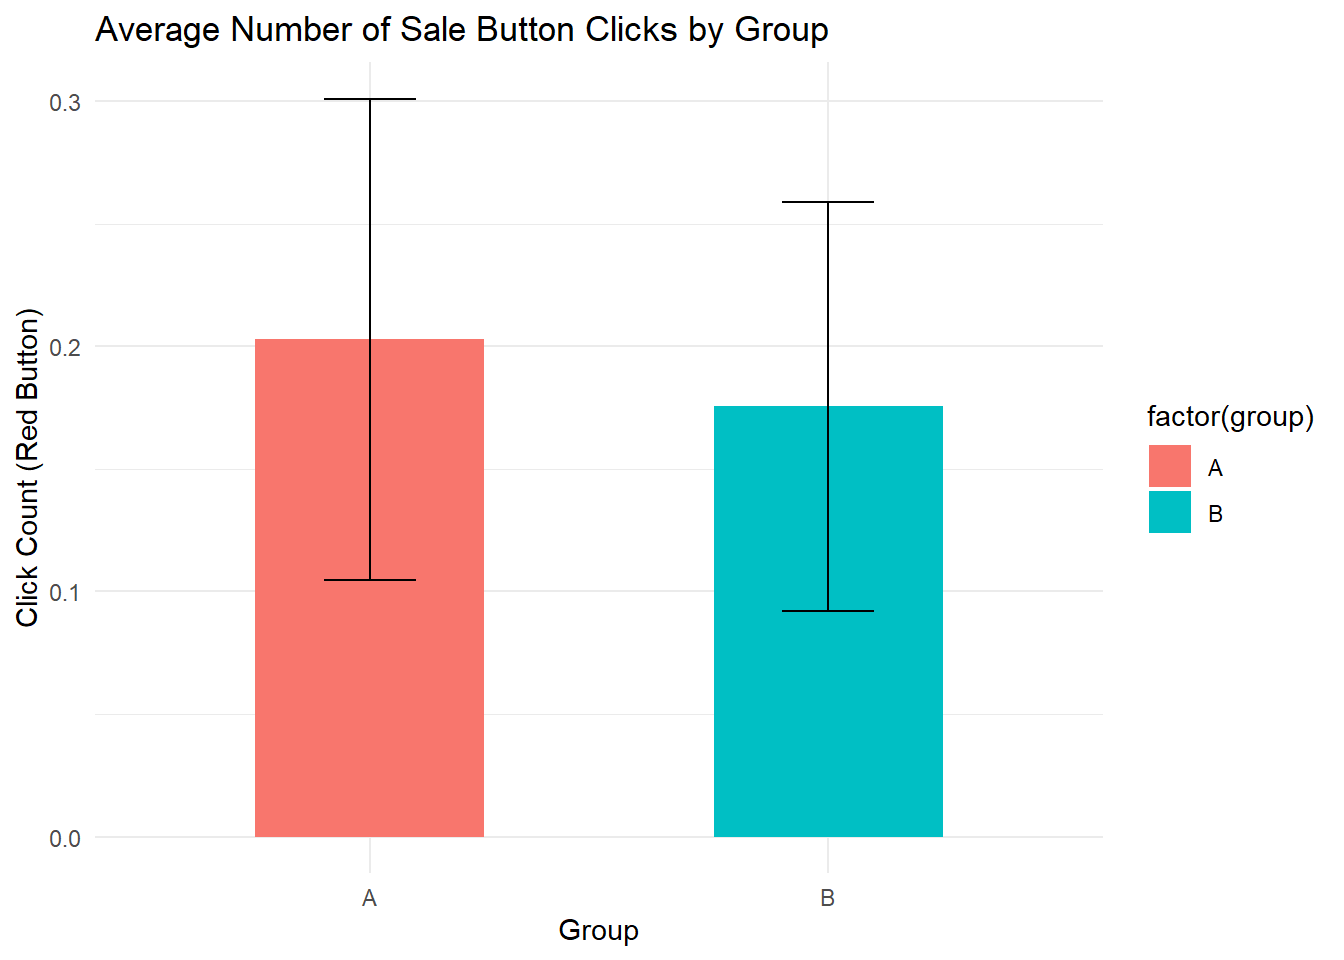
\includegraphics[width=0.7\textwidth,height=\textheight]{data_ana_pj3_files/figure-html/unnamed-chunk-3-1.png}
\end{center}
\\

From the plot above, we observe that Group A users had a slightly higher
average number of clicks (0.203) compared to Group B users (0.175).
While this suggests a marginal increase in engagement under the red
button condition, the visual difference was small and warranted
statistical testing to determine its significance.

To assess the statistical validity of this difference, we performed a
Welch two-sample t-test, which does not assume equal variances.\\

\begin{center}
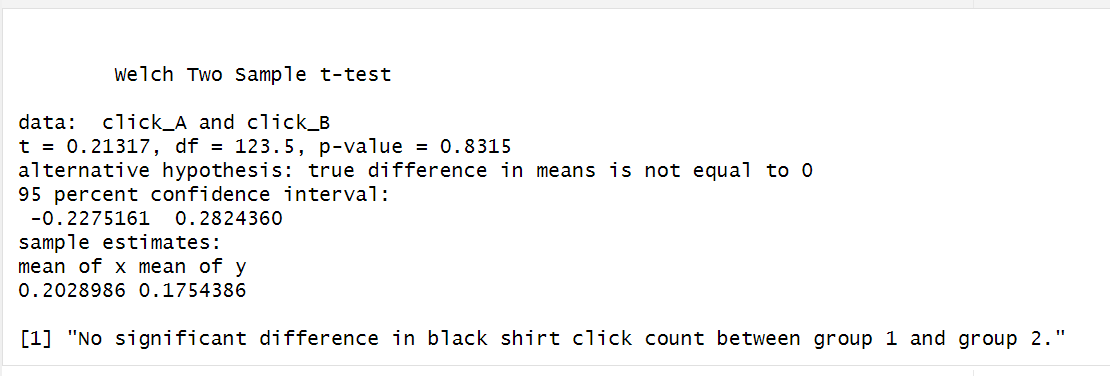
\includegraphics[width=0.7\textwidth,height=\textheight]{data_ana_pj3_files/t_test_result.png}
\end{center}
\\

The test yielded a t-statistic of 0.213 and a p-value of 0.8315. The
95\% confidence interval for the mean difference ranged from -0.2275 to
0.2824. Since the p-value far exceeds the typical alpha level of 0.05,
we fail to reject the null hypothesis and conclude that the observed
difference in click counts between the two groups is not statistically
significant.

Next, we transformed the click data into a binary indicator---1 if the
user clicked at least once, 0 otherwise---to examine group-level
differences in click-through likelihood. We then conducted a chi-square
test of independence.

\begin{center}
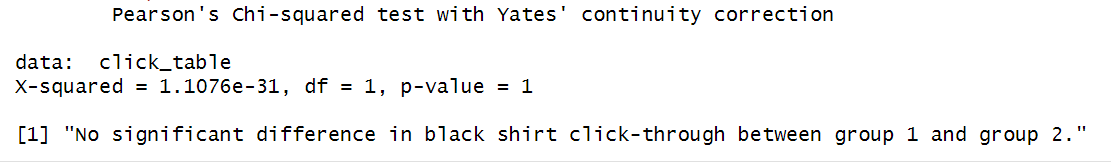
\includegraphics[width=0.7\textwidth,height=\textheight]{data_ana_pj3_files/chi_square.png}
\end{center}
\\
The chi-square test returned a statistic close to zero with a p-value of
1.0, indicating no statistically significant association between group
assignment and whether a user clicked the sale button. We suspect this
may be partially attributed to the low click frequency in both groups.

To account for the small sample size, we conducted a two-sample
proportion test. In Group A, 6 out of 69 users clicked the button
(≈8.70\%), while in Group B, 5 out of 57 users clicked (≈8.77\%). The
proportion test yielded a p-value of 0.988 and a 95\% confidence
interval ranging from -0.0998 to 0.0983. These results confirm that
there is no statistically significant difference in the proportion of
users clicking between the two button color conditions.

Following best practices for small cell counts, we additionally ran a
Fisher's Exact Test.

\begin{figure}[H]

{\centering 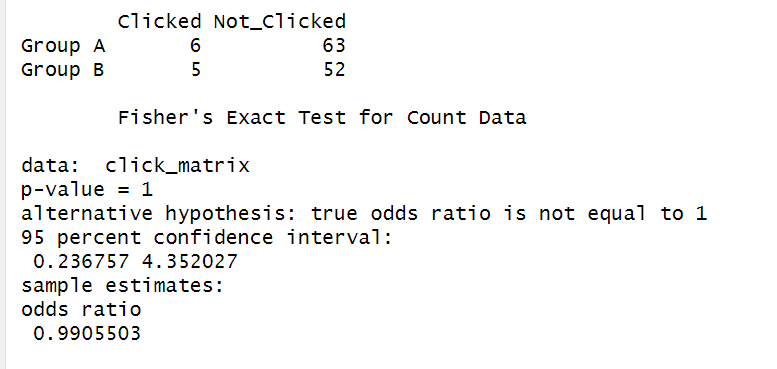
\includegraphics[width=0.7\textwidth,height=\textheight]{data_ana_pj3_files/fisher.png}

}

\caption{Fisher test result}

\end{figure}%%
\begin{figure}[H]

{\centering 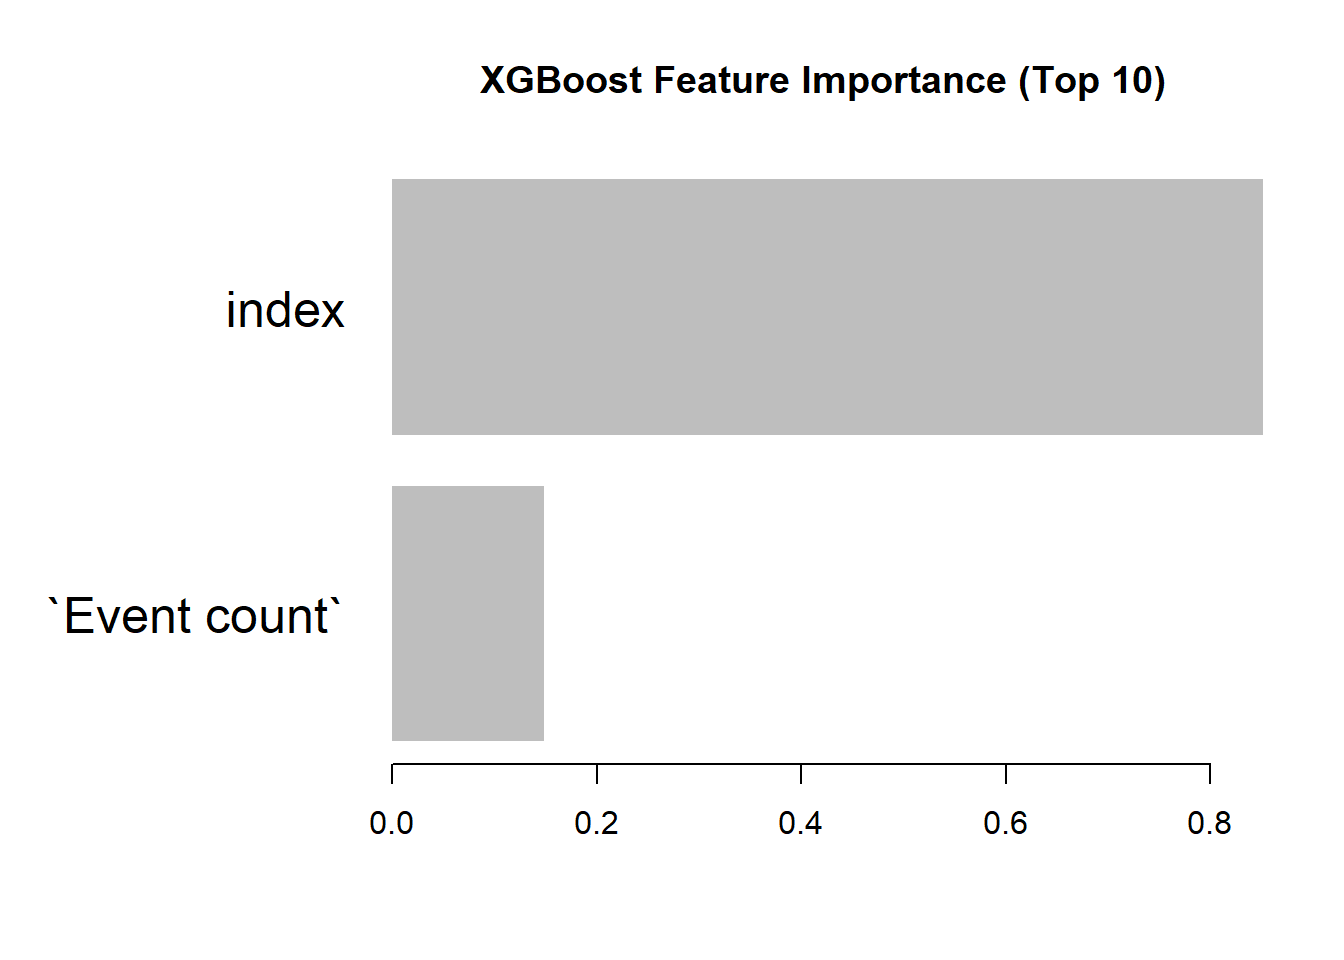
\includegraphics[width=0.7\textwidth,height=\textheight]{data_ana_pj3_files/figure-html/unnamed-chunk-7-1.png}

}

\caption{Fisher result}

\end{figure}%

This test produced a p-value of 1.0 and an odds ratio of approximately
0.99, with a wide confidence interval. The results reaffirmed previous
findings and further supported the conclusion that group assignment had
no significant influence on click behavior.

To complement our hypothesis tests with a predictive modeling
perspective, we trained an XGBoost binary classifier to predict whether
a user clicked the black shirt button based on session-level features
recorded from Google Analytics. These features included metrics such as
total event count, session duration, engagement rate, and group
assignment.\\
\begin{center}
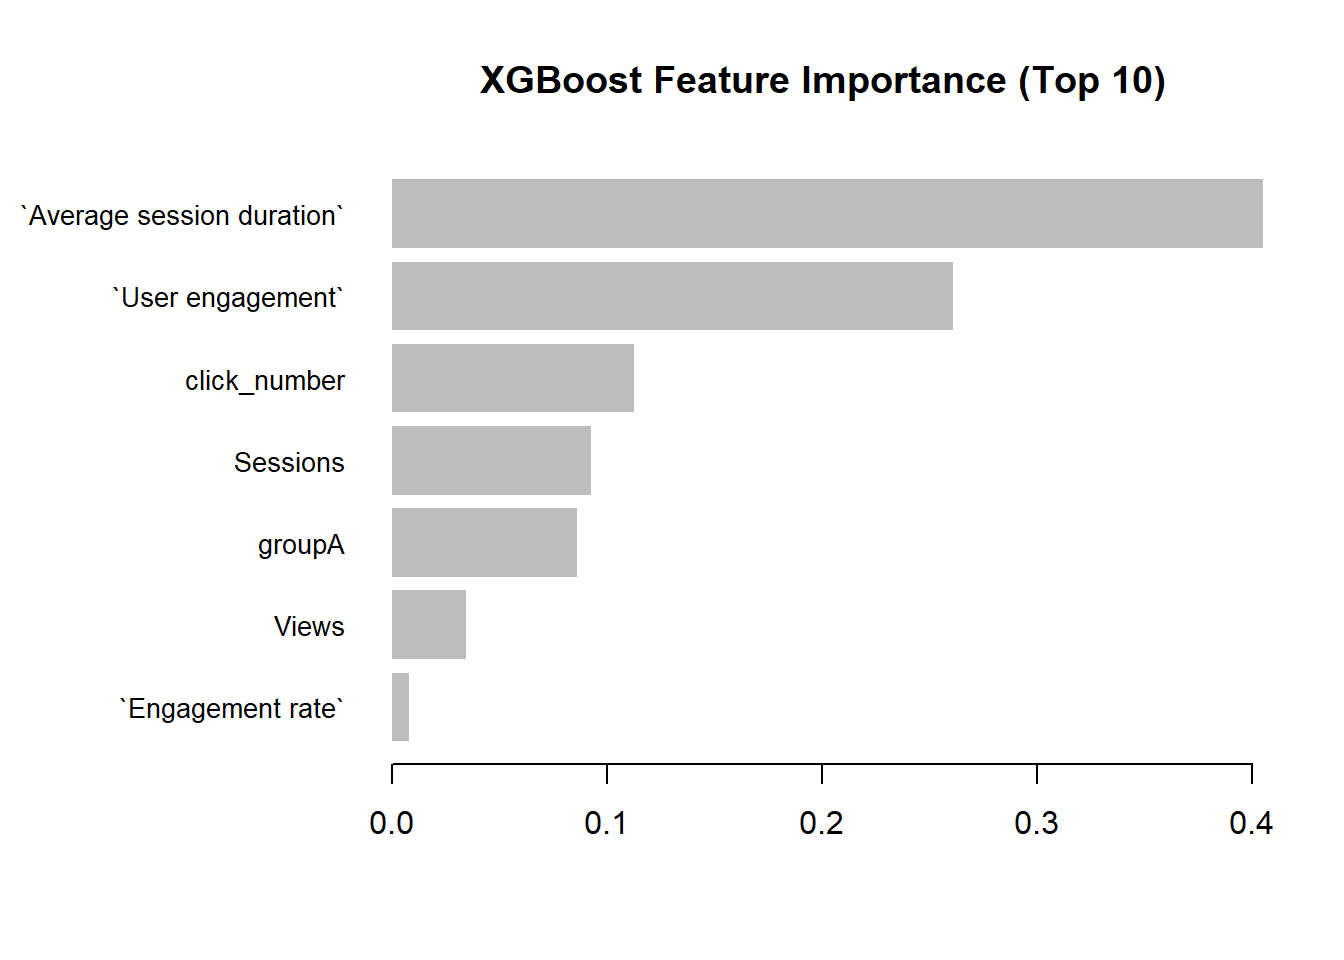
\includegraphics[width=0.7\textwidth,height=\textheight]{data_ana_pj3_files/figure-html/unnamed-chunk-8-1.png}
\end{center}
\\
From the result, we can tell the Average session duration, User
engagement, and the Click Number are the top three most important
factors. However, the group variable (groupA) has relatively low
importance in the model, which is consistent with our earlier
statistical tests (t-test, chi-square, and fisher test) showing no
significant difference in click rates between Group A and Group B.\\

To further interpret our XGBoost model, we generated Partial Dependence
Plots (PDP) to investigate one of the most important factors-
click\_number affects the likelihood of a user clicking the buy
button.\\
\begin{center}
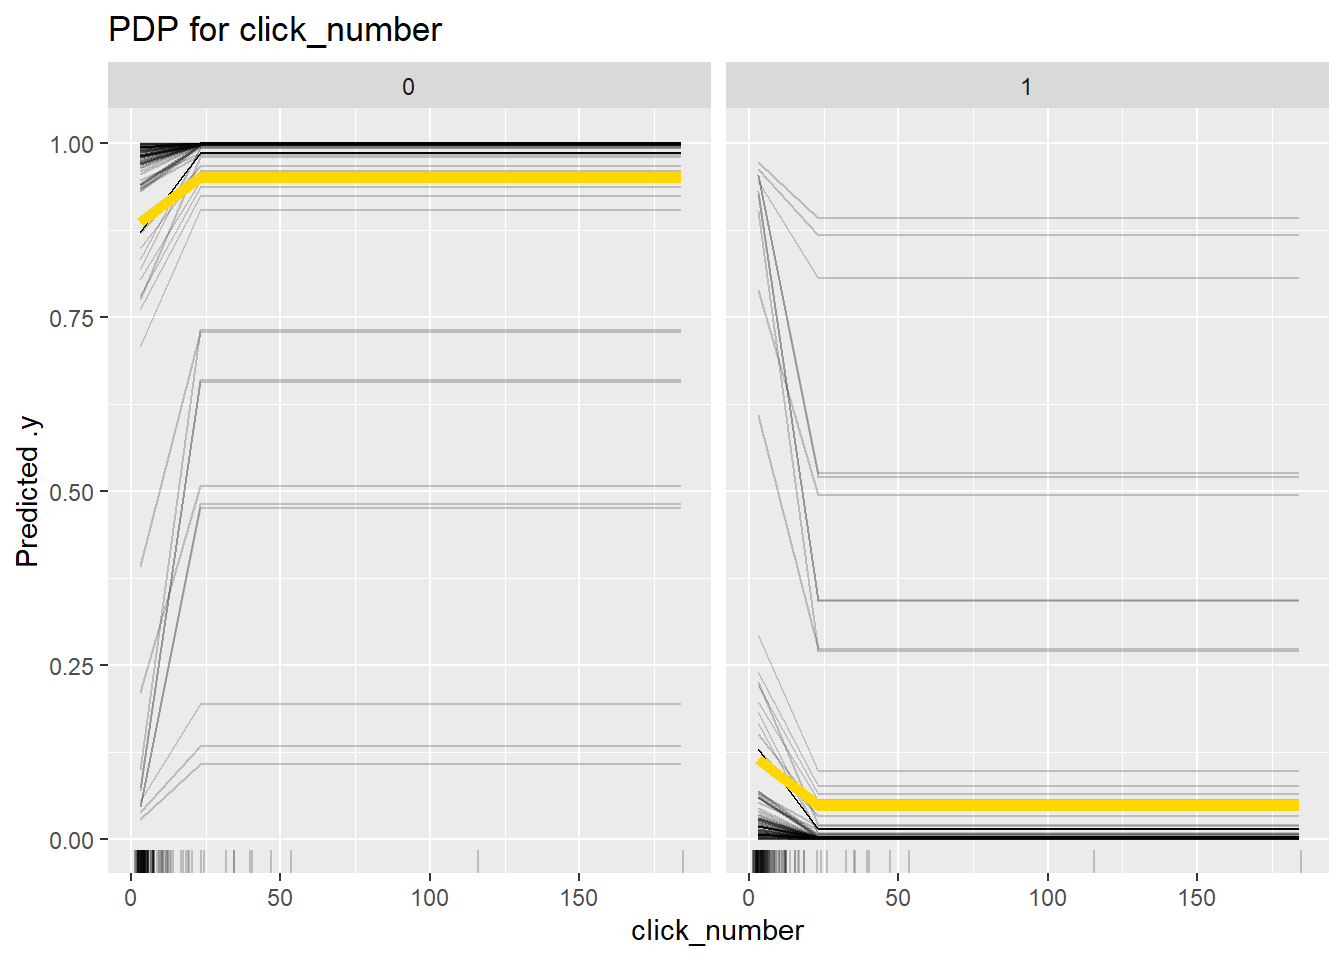
\includegraphics[width=0.7\textwidth,height=\textheight]{data_ana_pj3_files/figure-html/unnamed-chunk-9-1.png}
\end{center}
\\
To explore interaction effects between click\_number and group
assignment, we also generated a 2D PDP plot: \begin{center}
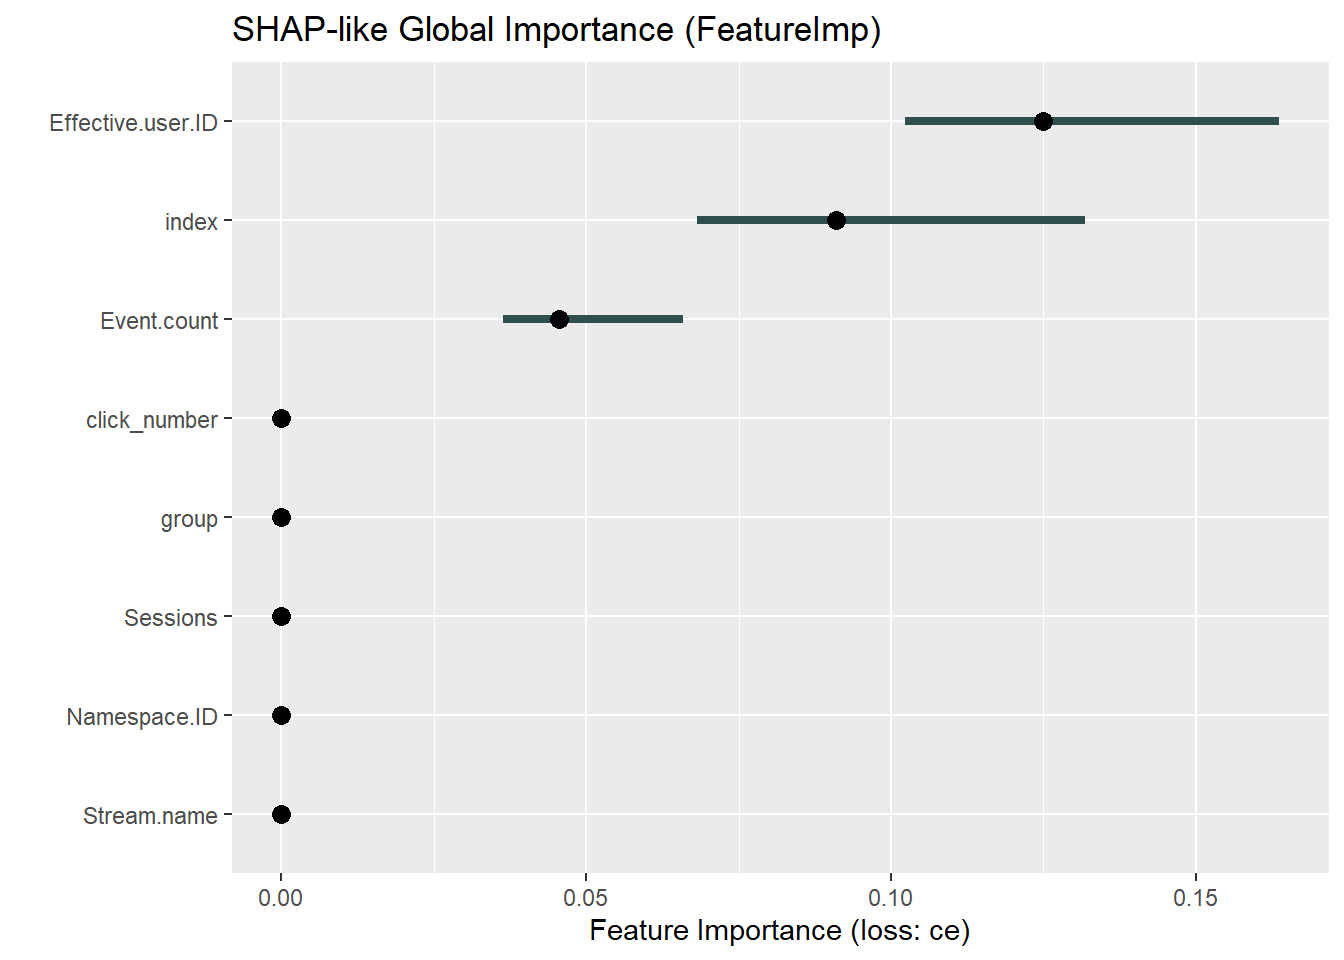
\includegraphics[width=0.7\textwidth,height=\textheight]{data_ana_pj3_files/figure-html/unnamed-chunk-9-2.png}
\end{center}
\\
The interaction plot shows that for both groups A and B, the predicted
probability of purchase remains consistently low regardless of
click\_number. This pattern confirms that, while click\_number plays a
role in model prediction individually, its interaction with the group
assignment does not lead to significant changes. The group is neither
direly related to the clicking sale button, nor does it related to the
click number.\\

We applied SHAP (SHapley Additive exPlanations) to evaluate the
contribution of each feature to the prediction of whether a user clicked
the purchase button.

We first generated a local SHAP explanation for a single user:\\
\begin{center}
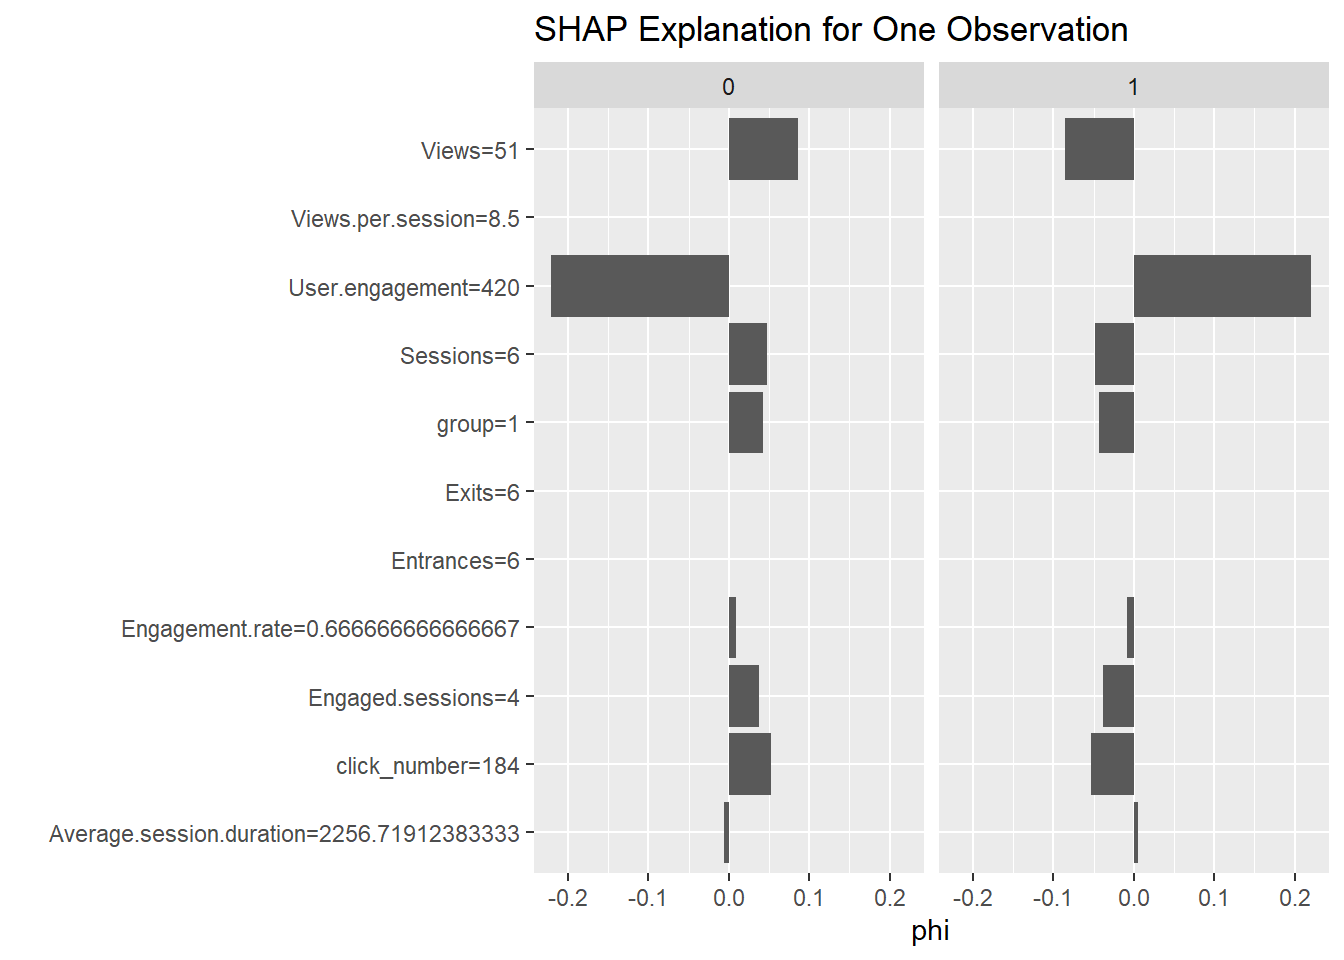
\includegraphics[width=0.7\textwidth,height=\textheight]{data_ana_pj3_files/figure-html/unnamed-chunk-10-1.png}
\end{center}
\\
This specific user had high user engagement and session counts, which
contributed positively toward the predicted probability of clicking the
button.

Then, we used the Feature Imp method to compute a global SHAP-like
feature importance across all users:\\
\begin{center}
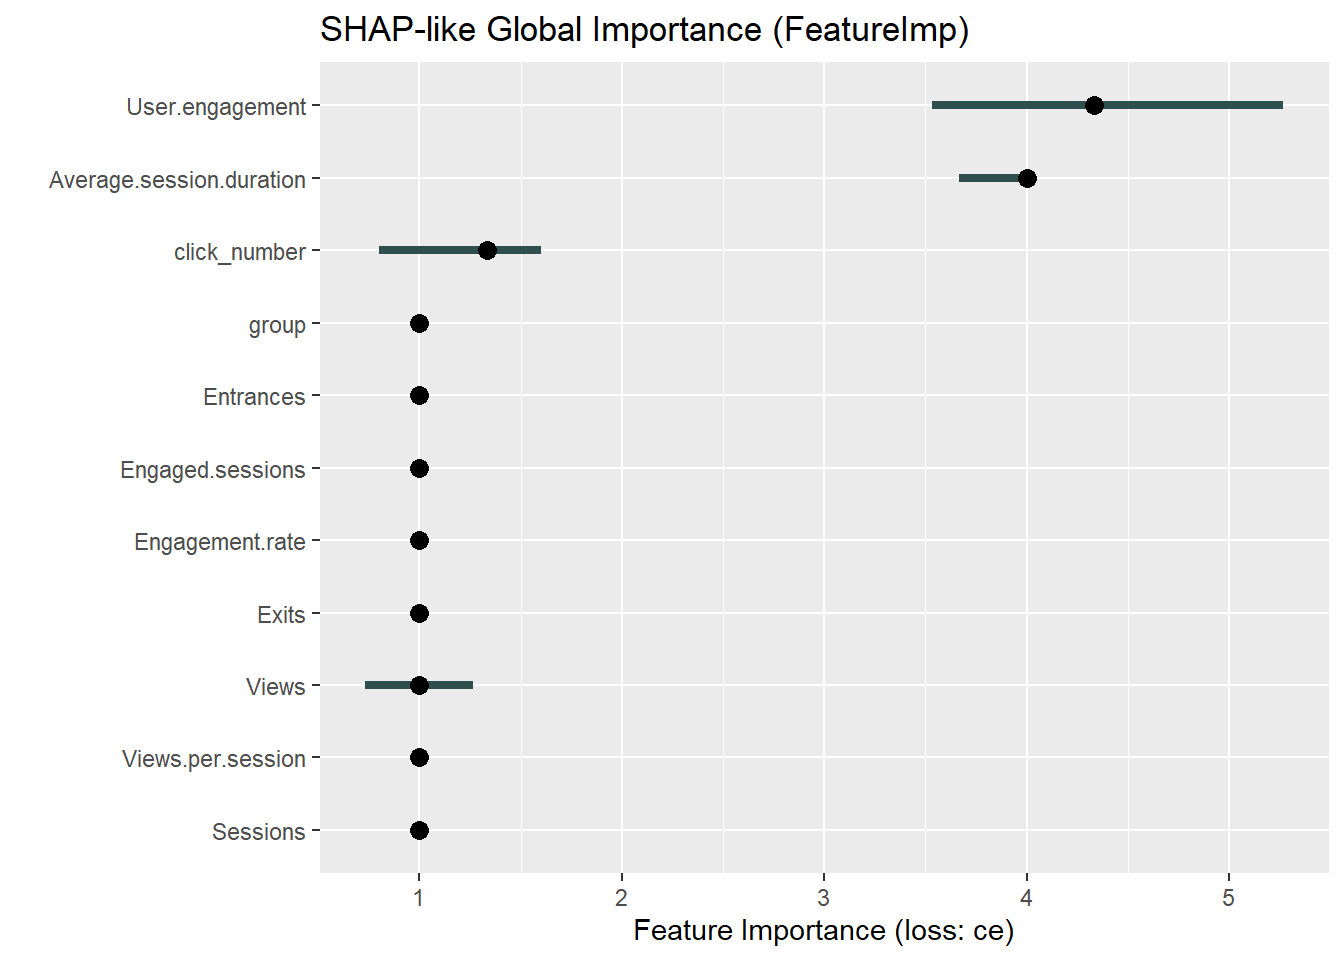
\includegraphics[width=0.7\textwidth,height=\textheight]{data_ana_pj3_files/figure-html/unnamed-chunk-10-2.png}
\end{center}
\\
From this result, we can tell that User engagement and Average session
duration are the most important features globally for the model, and the
group difference has no contribution towards the clicks for the sale
button.\\

we visualized the distribution of SHAP values for each feature using
violin plots to further explore the feature-level differences between
group A and group B. As shown below, certain variables such as
click\_number, User.engagement, and Engaged.sessions demonstrated
noticeable divergence in SHAP contributions between the two groups.\\
\begin{center}
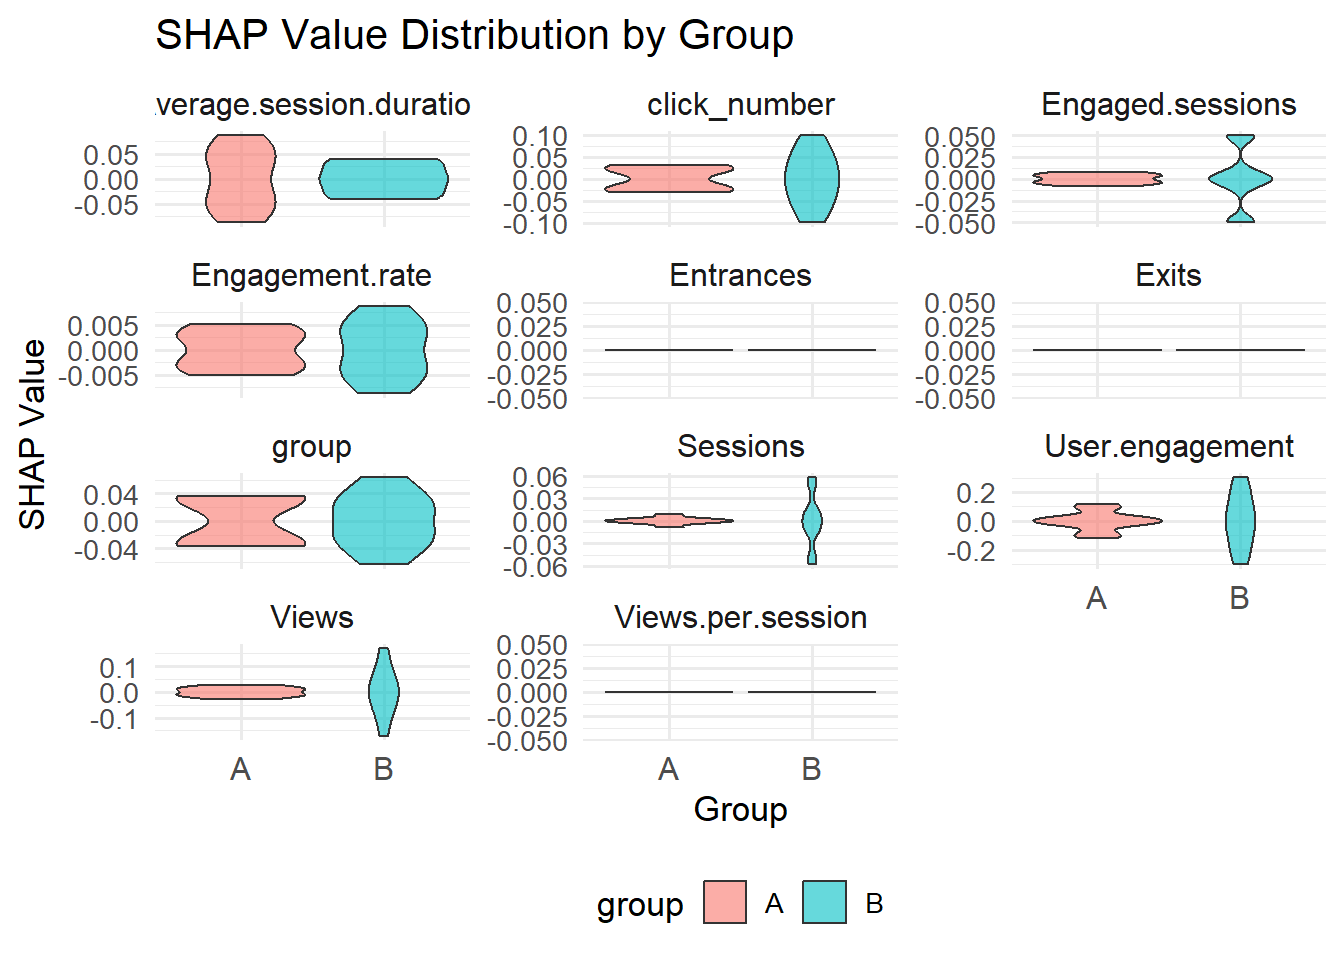
\includegraphics[width=0.7\textwidth,height=\textheight]{data_ana_pj3_files/figure-html/unnamed-chunk-12-1.png}
\end{center}
\\
For instance, click\_number appears to have a wider SHAP range in group
B, which means this feature plays a more substantial role in driving
prediction shifts for group B. On the other hand, features like Exits
and Entrances exhibit nearly flat SHAP distributions for both groups.

\begin{itemize}
\tightlist
\item
  \textbf{Interpretation \& Conclusion}
\end{itemize}

In conclusion, the group difference---namely the use of a red color for
the sales button---does not appear to have a statistically significant
impact on users' tendency to click the purchase button. Instead,
features such as average session duration, user engagement, and click
number show stronger predictive power in influencing user behavior.

However, slight variations in SHAP values for user engagement and click
number between the two groups suggest that the red color might still
have a subtle effect on user interaction. This implies that while the
red button alone is not a dominant factor, it may contribute marginally
to the overall clicking behavior.\\

\begin{itemize}
\tightlist
\item
  \textbf{Challenges \& Limitations}
\end{itemize}

\begin{verbatim}
-   Google Analytics data take longer time to update at around 24-48 hours, so we need to wait until we get the data we want.

-   The file google-analytics.html was first designed with a tag event_name "purchase_click" for all shirt items, with different event_label 'Plain Black Shirt (Sale)', 'Code Shirt', and 'Graphic Shirt'. However, we later realized that it was difficult to retreived the data for event_label separately, so we change to incorporate all details in event_name which are 'purchase_click_plain_black_shirt_sale,' 'purchase_click_code_shirt' and 'purchase_click_graphic_shirt'.

-   The cookie-based assignment did not work properly, as a different version of the website would sometimes appear on subsequent clicks, so we added a small delay (100ms) to ensure the cookie is saved before the page redirects.
\end{verbatim}

\begin{itemize}
\item
  \textbf{Contribution:}

  Hanzhong Yang (hy2870): Coding for Statistical Analysis,Statistical
  Analysis, Statistical Results, Report drafting

  Preach Apintanapong (pa2615): Formal website building, Google
  Analytics building, Report drafting

  Mengyan Li (ml4779): Original website building, User Explorer
  Building, Report drafting

  Raymond Li (jl6787): Some Coding for Statistical Analysis, Report
  refining.
\item
  ** Github Link:**
  https://github.com/My990813/Applied-Data-Science-Project-Three
\end{itemize}




\end{document}
